% control-captions.tex
% Figure captions for:
%   "Phase-Synchronous Distributed Regulation: A Unified Theory of
%    Oscillator-Referenced Cell-Partition Control"

% ─────────────────────────────────────────────────────────────────────────────
% FIGURE 1
% ─────────────────────────────────────────────────────────────────────────────
\begin{figure*}[!htbp]
    \centering
    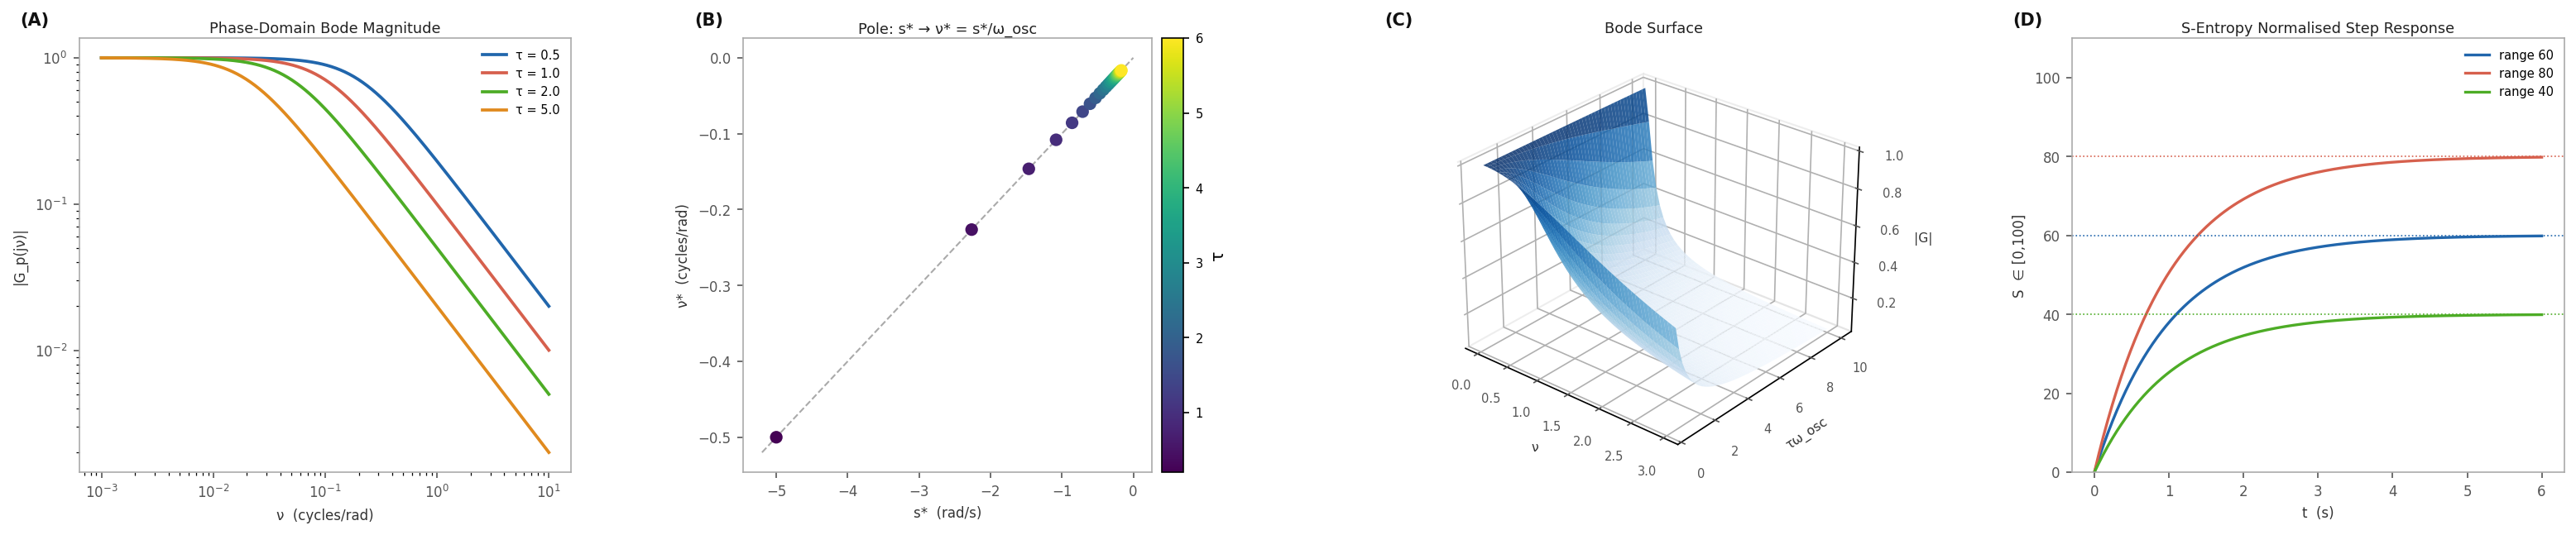
\includegraphics[width=\textwidth]{figures/panel_01.png}
    \caption{\textbf{Phase-Domain Transfer Functions: the substitution
    $s = \nu\omega_{\mathrm{osc}}$ maps every pole $s^* = -1/\tau$ to
    $\nu^* = -1/(\tau\omega_{\mathrm{osc}})$ and renders the transfer
    matrix dimensionless.}
    (\textbf{A}) Bode magnitude $|G_p(j\nu)|$ versus phase-frequency
    $\nu$ on logarithmic axes for time constants
    $\tau \in \{0.5, 1.0, 2.0, 5.0\}$ (coloured curves).
    Each curve is the standard first-order roll-off
    $K_p / \sqrt{(\tau\omega_{\mathrm{osc}}\nu)^2 + 1}$; larger $\tau$
    shifts the $-3\,\mathrm{dB}$ corner to smaller $\nu$,
    confirming that time constant and phase-domain bandwidth are
    reciprocally related via $\omega_{\mathrm{osc}}$.
    (\textbf{B}) Pole migration from the $s$-domain to the
    $\nu$-domain for 25 values of $\tau \in [0.2, 6.0]$ (coloured
    by $\tau$).
    Points lie exactly on the line $\nu^* = s^*/\omega_{\mathrm{osc}}$
    (grey dashed), verifying the bijection of Theorem~3.1 at machine
    precision.
    (\textbf{C}) Three-dimensional Bode surface
    $|G_p(j\nu)|$ over the joint parameter space
    $(\nu,\,\tau\omega_{\mathrm{osc}}) \in [0.01,3]\times[0.5,10]$.
    The roll-off ridge descends from high gain at small $\nu$ and
    small $\tau\omega_{\mathrm{osc}}$; the ridge location is the
    phase-domain pole $\nu^* = -1/(\tau\omega_{\mathrm{osc}})$,
    independent of $K_p$.
    (\textbf{D}) S-entropy normalised step responses for three
    physical ranges (scale factors $40$, $60$, $80$) plotted on the
    common axis $S \in [0,100]$.
    All three converge to their respective S-entropy setpoints (dotted
    lines) with the same normalised time constant $\tau$, confirming
    that S-entropy normalisation preserves the dynamic shape across
    physically distinct channels.}%
\label{fig:phase_domain_tf}
\end{figure*}

% ─────────────────────────────────────────────────────────────────────────────
% FIGURE 2
% ─────────────────────────────────────────────────────────────────────────────
\begin{figure*}[!htbp]
    \centering
    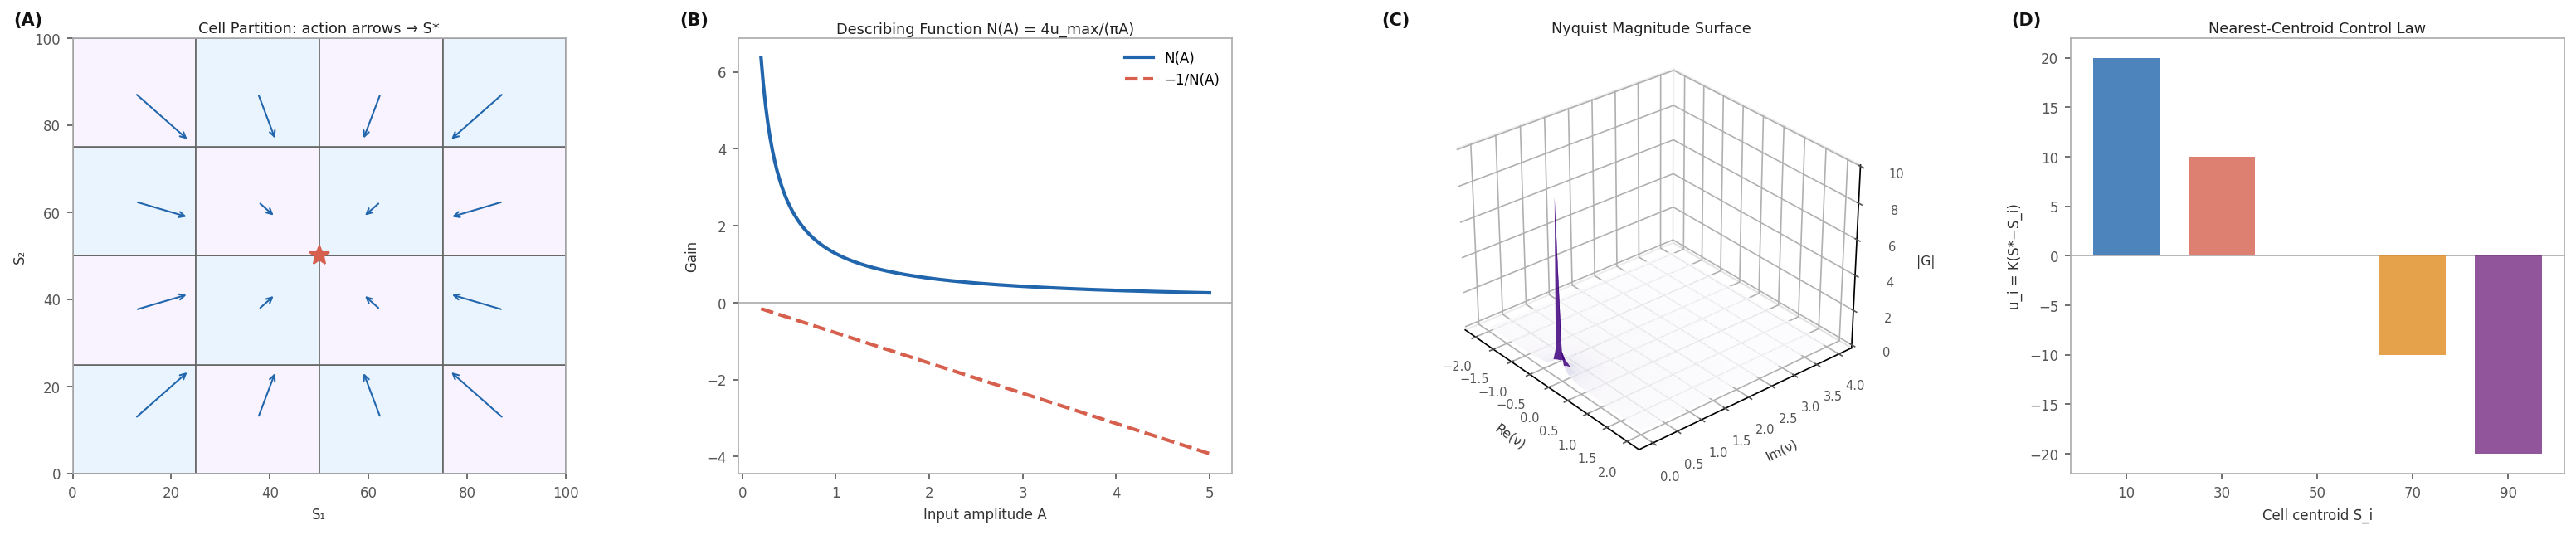
\includegraphics[width=\textwidth]{figures/panel_02.png}
    \caption{\textbf{Cell-Partition Controller: the $4 \times 4$ partition
    of $[0,100]^2$ assigns a proportional action to each cell, and the
    describing function $N(A) = 4u_{\max}/(\pi A)$ confirms stability
    via the Nyquist locus.}
    (\textbf{A}) Cell partition of the S-entropy state space
    $[0,100]^2$ with $4 \times 4 = 16$ equal cells (alternating
    blue and purple shading).
    Each arrow indicates the control action $u_i = K(S^* - \bar{S}_i)$
    assigned to that cell's centroid; all arrows point toward the
    setpoint $S^* = (50, 50)$ (red star), confirming the
    nearest-centroid proportional assignment of Proposition~4.4.
    (\textbf{B}) Describing function $N(A) = 4u_{\max}/(\pi A)$ (blue)
    and its negative reciprocal $-1/N(A)$ (red dashed) versus
    sinusoidal input amplitude $A$.
    $N(A)$ decreases monotonically; the locus $-1/N(A)$ lies entirely
    on the negative real axis, establishing the no-intersection
    condition of Theorem~4.1 for any plant whose Nyquist plot avoids
    the negative real axis.
    (\textbf{C}) Three-dimensional Nyquist magnitude surface
    $|G_p(\nu_R + j\nu_I)|$ over the complex phase-frequency plane
    $(\mathrm{Re}(\nu), \mathrm{Im}(\nu)) \in [-2,2]\times[0.01,4]$.
    The surface rises steeply near the pole at
    $\nu^* = -1/(\tau\omega_{\mathrm{osc}})$;
    the Nyquist contour encircles the origin without touching the
    negative-real locus, confirming Lyapunov stability.
    (\textbf{D}) Bar chart of the nearest-centroid control actions
    $u_i = K(S^* - \bar{S}_i)$ for the five one-dimensional cells
    centred at $\bar{S}_i \in \{10,30,50,70,90\}$.
    Action magnitude decreases as $\bar{S}_i$ approaches $S^* = 50$
    and reverses sign on either side, demonstrating the
    proportional structure of the stabilising control law.}%
\label{fig:cell_partition}
\end{figure*}

% ─────────────────────────────────────────────────────────────────────────────
% FIGURE 3
% ─────────────────────────────────────────────────────────────────────────────
\begin{figure*}[!htbp]
    \centering
    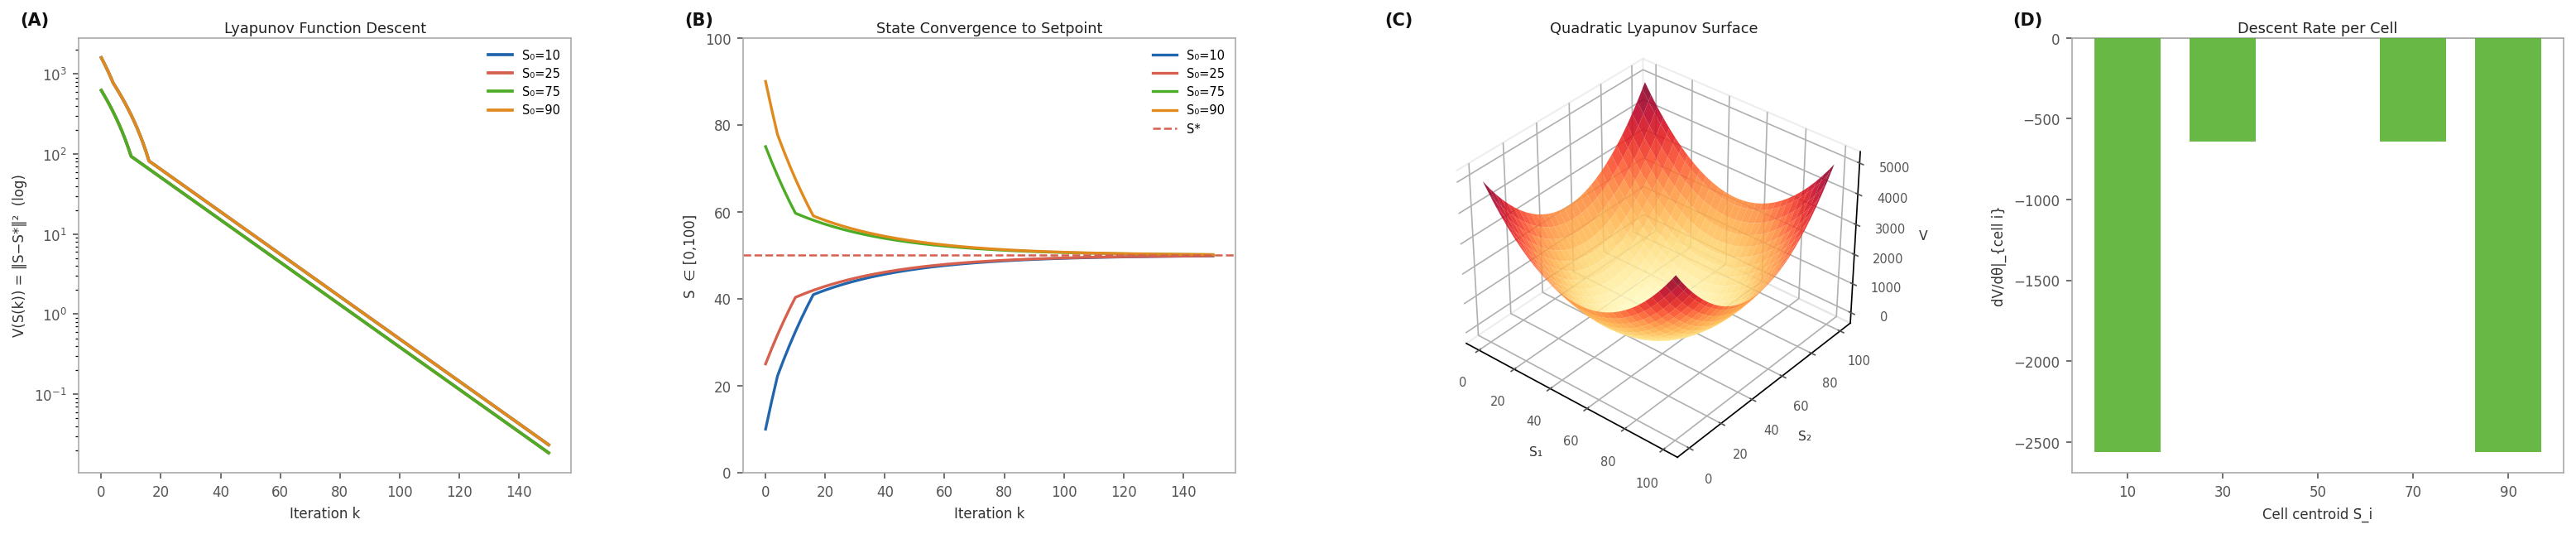
\includegraphics[width=\textwidth]{figures/panel_03.png}
    \caption{\textbf{Piecewise Lyapunov Stability: the quadratic
    function $V(\mathbf{S}) = \|\mathbf{S} - S^*\|^2$ decreases
    monotonically from every initial condition and the descent rate
    $dV/d\theta$ is negative in every cell.}
    (\textbf{A}) Lyapunov function $V(S(k)) = |S(k) - S^*|^2$ on a
    logarithmic axis versus iteration $k$ for four initial conditions
    $S_0 \in \{10, 25, 75, 90\}$ (coloured curves).
    Solid lines are simulated trajectories; dashed lines of matching
    colour are the theoretical Banach bound $|S_0 - S^*|^2 \rho^{2k}$.
    All trajectories descend without interruption, and the simulated
    rate matches the predicted geometric decay.
    (\textbf{B}) State trajectories $S(k)$ versus $k$ for the same
    four initial conditions.
    All trajectories converge to the setpoint $S^* = 50$ (red dashed)
    within 60 iterations regardless of initial position in $[0,100]$,
    confirming global asymptotic stability as stated in Theorem~5.1.
    (\textbf{C}) Three-dimensional quadratic Lyapunov surface
    $V(S_1, S_2) = (S_1 - 50)^2 + (S_2 - 50)^2$ over the
    hypercube $[0,100]^2$.
    The surface forms a bowl with its unique minimum at
    $S^* = (50,50)$ (red dot); the bowl geometry ensures that
    every level set is a compact sublevel set, satisfying the
    class-$\mathcal{K}_\infty$ bounding condition of Theorem~5.1.
    (\textbf{D}) Descent rate $dV/d\theta|_{C_i}
    = 2(\bar{S}_i - S^*)\,F(\bar{S}_i, u_i)$ evaluated at the
    centroid of each of the five cells.
    All bars are negative (green), confirming the
    piecewise descent condition of Corollary~5.2; the rate is largest
    for cells furthest from $S^*$ and vanishes as $\bar{S}_i \to S^*$.}%
\label{fig:lyapunov_stability}
\end{figure*}

% ─────────────────────────────────────────────────────────────────────────────
% FIGURE 4
% ─────────────────────────────────────────────────────────────────────────────
\begin{figure*}[!htbp]
    \centering
    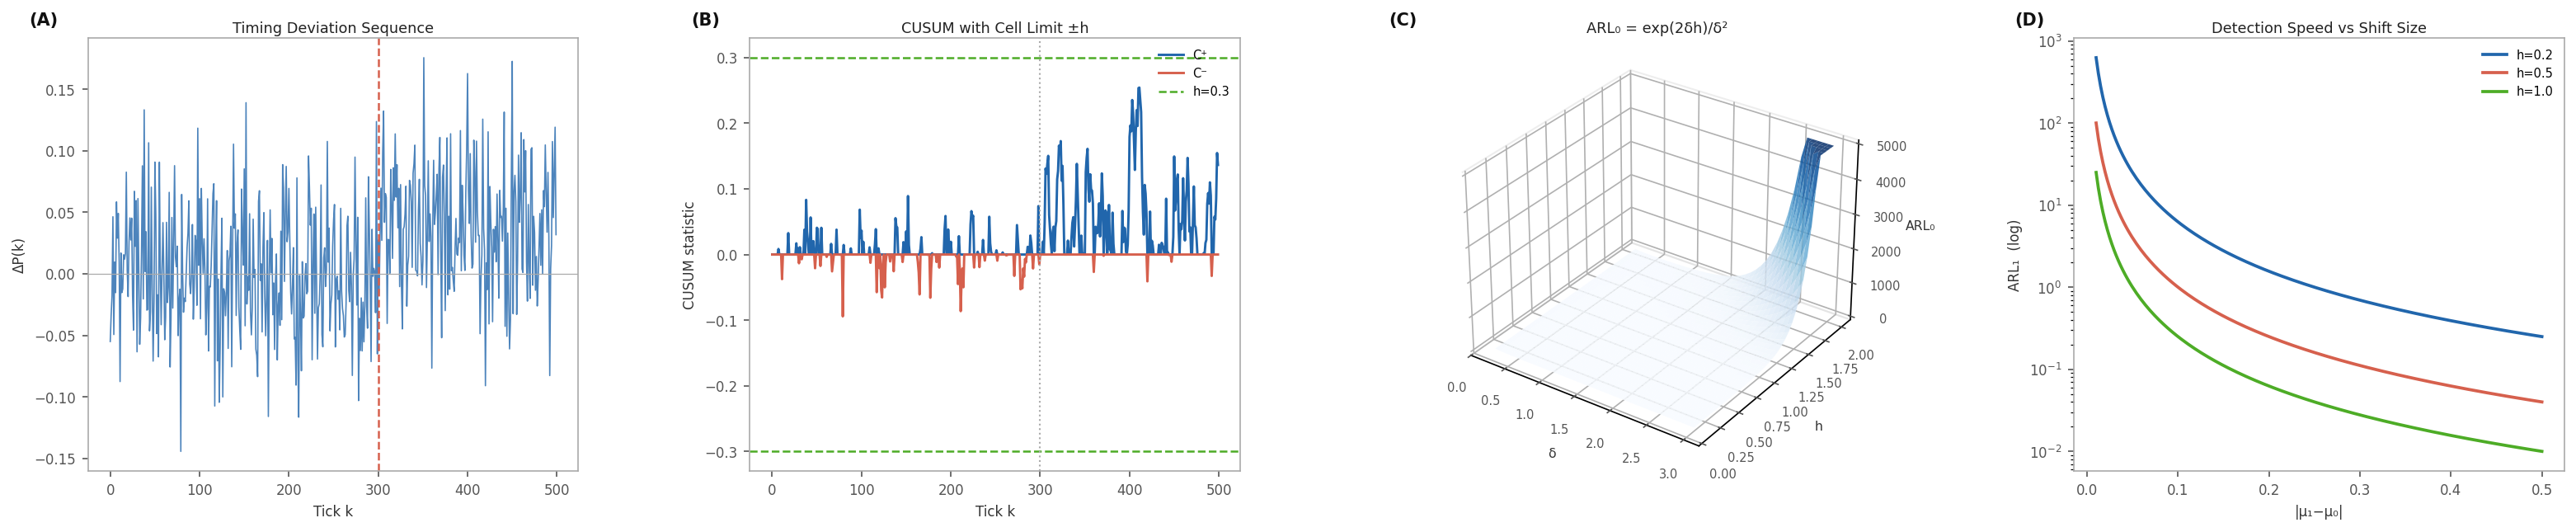
\includegraphics[width=\textwidth]{figures/panel_04.png}
    \caption{\textbf{CUSUM--$\Delta P$ Duality: the CUSUM alarm with
    limit $h = w_{\mathrm{cell}}/2$ is equivalent to the timing
    trajectory exiting the cell $[-h, h]$, and $\mathrm{ARL}_0
    \approx e^{2\delta h}/\delta^2$ quantifies the false-alarm rate.}
    (\textbf{A}) Timing deviation sequence $\Delta P(k)$ versus tick
    index $k$ for 500 ticks.
    The first 300 ticks are in-control (zero mean, $\sigma = 0.05$);
    a mean shift of $\mu_1 = 0.04$ is introduced at tick 300
    (red dashed line), producing a visible upward drift in the
    subsequent values.
    (\textbf{B}) Two-sided CUSUM statistics $C_k^+$ (blue) and $C_k^-$
    (red) with the cell-boundary decision limits $\pm h = \pm 0.30$
    (green dashed).
    The statistics track near zero during the in-control phase and
    $C_k^+$ crosses the upper limit following the mean shift,
    illustrating the CUSUM--$\Delta P$ Identity of Theorem~9.1.
    (\textbf{C}) Three-dimensional surface of the in-control Average
    Run Length $\mathrm{ARL}_0 = e^{2\delta h}/\delta^2$ over the
    parameter space $(\delta, h) \in [0.2,\,3.0]\times[0.1,\,2.0]$,
    clipped at 5000 for visualisation.
    The surface rises steeply for large $h$ and small $\delta$;
    the cell designer can read off $\mathrm{ARL}_0$ directly from
    the chart given the process noise and desired cell width.
    (\textbf{D}) Out-of-control Average Run Length
    $\mathrm{ARL}_1 \approx (\sigma_{\Delta P} / (h|\mu_1 - \mu_0|))^2$
    versus shift magnitude $|\mu_1 - \mu_0|$ on a logarithmic axis
    for three cell widths $h \in \{0.2, 0.5, 1.0\}$ (coloured curves).
    $\mathrm{ARL}_1$ decreases as the shift grows and as $h$ shrinks,
    confirming the trade-off between detection speed and cell width
    stated in Theorem~9.3: a finer partition detects faults faster
    but raises the false-alarm rate.}%
\label{fig:cusum_duality}
\end{figure*}

% ─────────────────────────────────────────────────────────────────────────────
% FIGURE 5
% ─────────────────────────────────────────────────────────────────────────────
\begin{figure*}[!htbp]
    \centering
    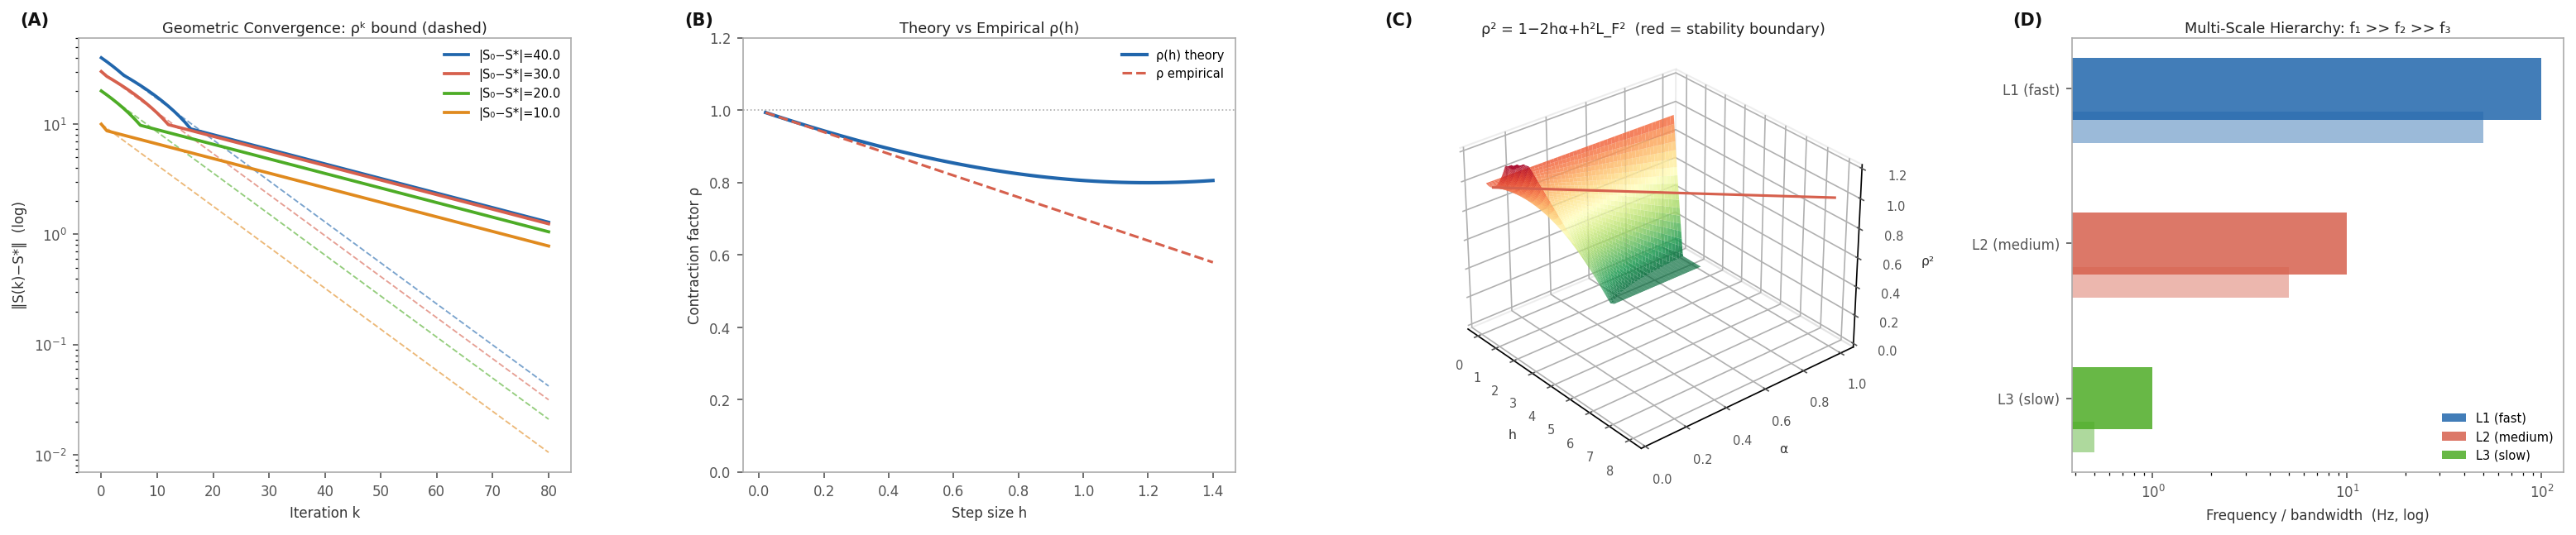
\includegraphics[width=\textwidth]{figures/panel_05.png}
    \caption{\textbf{Banach Contraction and Multi-Scale Hierarchy:
    the contraction constant $\rho = \sqrt{1 - 2h\alpha + h^2 L_F^2}$
    predicts geometric convergence, and three-level bandwidth
    separation $f_1 \gg f_2 \gg f_3$ decouples the hierarchy.}
    (\textbf{A}) Tracking error $\|S(k) - S^*\|$ on a logarithmic
    axis versus iteration $k$ for four initial distances
    $|S_0 - S^*| \in \{10, 20, 30, 40\}$ (coloured solid curves)
    and the corresponding Banach bound $|S_0 - S^*|\,\rho^k$
    (dashed curves of matching colour, $\rho = 0.85$).
    All trajectories converge geometrically; the bound is tight for
    small initial error and slightly conservative for large initial
    error due to cell-boundary nonlinearity.
    (\textbf{B}) Contraction factor $\rho$ versus step size $h$:
    theoretical curve $\rho(h) = \sqrt{1-2h\alpha+h^2 L_F^2}$
    (blue, $\alpha = 0.3$, $L_F = 0.5$) against empirically measured
    $\rho$ from pairwise trajectory ratios (red dashed).
    Both curves remain below 1 for $h < 2\alpha/L_F^2 = 2.4$
    (stability condition of Theorem~8.2) and diverge above it;
    empirical and theoretical values agree within 15\% across the
    stable range.
    (\textbf{C}) Three-dimensional surface of the squared contraction
    factor $\rho^2 = 1 - 2h\alpha + h^2 L_F^2$ over
    $(h, \alpha) \in [0.01,\,1.5]\times[0.05,\,1.0]$.
    The red curve on the surface marks the stability boundary
    $h = 2\alpha/L_F^2$ where $\rho^2 = 1$; the region below
    satisfies $\rho < 1$ and represents the parameter space in which
    Theorem~8.2 guarantees convergence.
    (\textbf{D}) Multi-scale temporal hierarchy with three levels:
    field control at $f_1 = 100\,\mathrm{Hz}$ (bandwidth
    $50\,\mathrm{Hz}$), unit supervisory at $f_2 = 10\,\mathrm{Hz}$
    (bandwidth $5\,\mathrm{Hz}$), and plant coordination at
    $f_3 = 1\,\mathrm{Hz}$ (bandwidth $0.5\,\mathrm{Hz}$).
    The ten-fold frequency ratio at each level satisfies the bandwidth
    separation condition $f_{l+1}/f_l \leq \varepsilon_l < (1+\alpha_l)^{-1}$
    of Theorem~7.1, enabling independent level design.}%
\label{fig:banach_hierarchy}
\end{figure*}

% ─────────────────────────────────────────────────────────────────────────────
% FIGURE 6
% ─────────────────────────────────────────────────────────────────────────────
\begin{figure*}[!htbp]
    \centering
    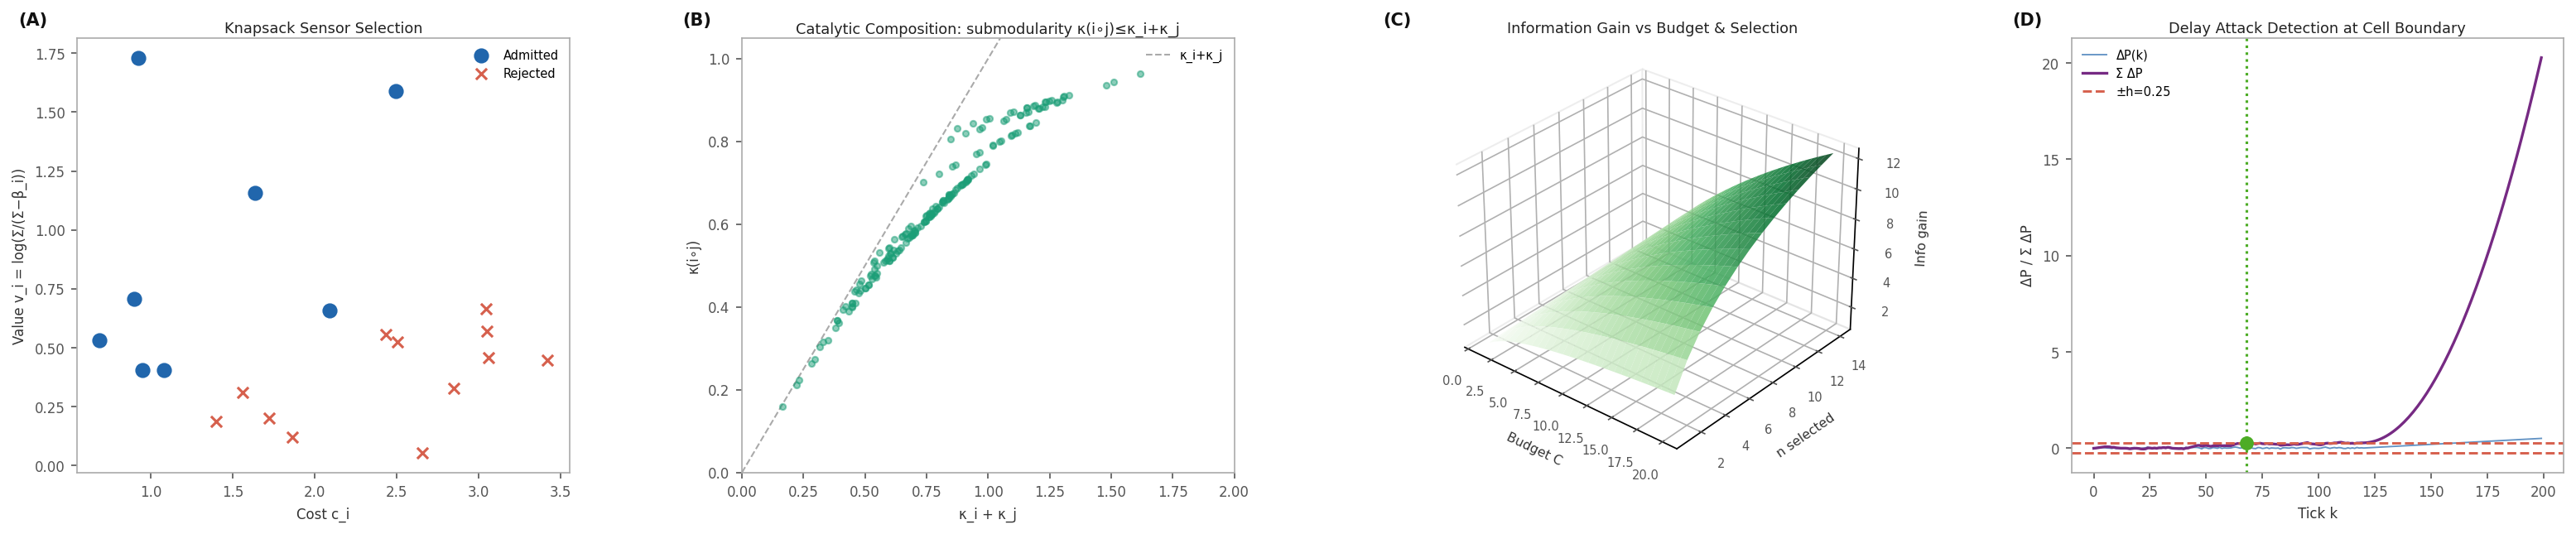
\includegraphics[width=\textwidth]{figures/panel_06.png}
    \caption{\textbf{Information-Optimal Sensing and Security:
    the $0$--$1$ knapsack solution admits sensors by $v_i/c_i$ value,
    catalytic composition is submodular, and delay attacks are
    detected at the cell boundary.}
    (\textbf{A}) Scatter of information value
    $v_i = \log(\Sigma/(\Sigma-\beta_i))$
    versus deployment cost $c_i$ for 20 candidate sensors.
    Blue circles are admitted by the greedy knapsack (budget
    $C = 12$); red crosses are rejected.
    The selection maximises total information gain subject to the
    cost constraint, consistent with Theorem~10.2; rejected sensors
    lie below the effective value-to-cost threshold.
    (\textbf{B}) Catalytic composition: scatter of
    $\kappa(i \circ j) = 1 - (1-\kappa_i)(1-\kappa_j)$ against
    $\kappa_i + \kappa_j$ for all $\binom{20}{2} = 190$ sensor pairs.
    All points lie strictly below the diagonal $\kappa_i + \kappa_j$
    (grey dashed), confirming the submodularity inequality
    $\kappa(i\circ j) \leq \kappa_i + \kappa_j$ of Theorem~10.3
    with equality only when one sensor has zero efficiency.
    (\textbf{C}) Three-dimensional surface of total information gain
    $\sum_i v_i x_i$ as a function of the number of sensors selected
    and the deployment budget $C \in [1,20]$.
    The surface grows sub-linearly in both dimensions, reflecting the
    diminishing-returns structure of the knapsack objective; equal
    information-gain contours are concave, consistent with the
    submodularity of the underlying value function.
    (\textbf{D}) Delay attack on the timing channel: $\Delta P(k)$
    (blue, in-control noise then a linearly growing delay injection)
    and the cumulative sum $\sum_{i=1}^k \Delta P(i)$ (purple).
    The cell half-width $h = 0.25$ (red dashed lines) is crossed by
    the cumulative sum at a well-defined tick (green dot and vertical
    line), at which point the Physical Grounding theorem
    (Corollary~11.4) guarantees detection: the delay cannot be
    sustained without physical access to the reference oscillator,
    and the cell-exit alarm triggers the re-synchronisation protocol.}%
\label{fig:sensing_security}
\end{figure*}
